%%%%%%%%%%%%%%%%%%%%%%%%%%%%%%%%%%%%%%%%%%%%%%%%%%%%%%%%%%%%%%%%%%%%%%%%%%%
\fancyChapter{Seeing Soft Materials Draped Over Objects}
[A Case Study of Intuitive Physics in Perception, Attention, and Memory]
\label{chap:PsychSci2023}
%%%%%%%%%%%%%%%%%%%%%%%%%%%%%%%%%%%%%%%%%%%%%%%%%%%%%%%%%%%%%%%%%%%%%%%%%%%

% Text copied from https://journals.sagepub.com/doi/10.1177/09567976221109194?url_ver=Z39.88-2003&rfr_id=ori:rid:crossref.org&rfr_dat=cr_pub%20%200pubmed

The human mind is highly attuned to regularities in the world around us \parencite{shepard_perceptual-cognitive_1994}, and surely some of the most universal regularities are the laws of physics. As such, psychologists have long been interested in how our minds may (or may not) incorporate physical principles, in the study of “intuitive physics” (for reviews, see \cite{kubricht_intuitive_2017, ullman_mind_2017}). Classic work, for example, demonstrated that when asked to draw the trajectory of a ball falling out of an airplane in mid-flight, most people fail to draw the correct parabolic paths (\cite{mccloskey_etal_1983}; see also \cite{mccloskey_curvilinear_1980}). And such effects generalize to real-world behavior: When asked to drop a ball (while walking) to hit a marked target on the floor, for example, many people release the ball when it is directly over the target, mistakenly predicting that it will fall straight down \parencite{mccloskey_alone_1983}.

Perhaps the two most salient themes from this work are (a) that people are often poor at reasoning about such phenomena (with many failing these tasks) and (b) that intuitive physics is centrally a matter of higher-level reasoning and decision-making. (Such errors are thought to stem from “erroneous beliefs” that are held “even after formal training in Newtonian mechanics”; \cite{kaiser_judgments_1985}, p.~795.)
The current project illustrates how these two themes provide an incomplete picture of how physical regularities are incorporated into the human mind and suggests that although people may often be poor at reasoning about physics, their visual percepts themselves reveal a surprising facility with physical principles (see also \cite{firestone_seeing_2017}). In short, we may often be poor at \textit{thinking} about physics, but we may nevertheless also be better at \textit{seeing} physics. (Of course, the distinction between visual processing and higher-level judgment can be drawn in many ways---e.g., involving automaticity, or stimulus-driven vs. task-dependent processing; for reviews, see \cite{block_border_2023, firestone_cognition_2016}. We aimed to design experiments that would speak broadly to such differences.) Here, we explored this experimentally in the context of what may at first seem like an unusual domain.

\begin{kaobox}[frametitle=Statement of Relevance]
    Many times per day, most of us see objects that are covered by soft materials -- e.g.~a chair with a blanket draped over it. Work in psychological science often starts with experiences like this that we take completely for granted but then shows how such experiences are supported by mental operations that are unexpectedly fascinating or complex. In this work we show that beyond how we may explicitly reason about such familiar layouts, our visual systems themselves infer unexpectedly sophisticated representations from such scenes, spontaneously extracting and highlighting the structure of the covered objects by taking into account subtle physical interactions between cloth, gravity, and object. This shows how the seemingly simple act of perceiving (and attending, and remembering) cloth-covered objects involves a surprisingly elaborate analysis of ``intuitive physics.''
\end{kaobox}

%%%%%%%%%%%%%%%%%%%%%%%%%%%%%%%%%%%%%%%%%%%%%%%%%%%%%%%%%%%%%%%%%%%%%%%%%%%
\section{``Cloth Physics''}
%%%%%%%%%%%%%%%%%%%%%%%%%%%%%%%%%%%%%%%%%%%%%%%%%%%%%%%%%%%%%%%%%%%%%%%%%%%

Intuitive physics is especially salient in phenomena involving colliding billiard balls or collapsing block towers (as reviewed by \cite{kubricht_intuitive_2017}) --- but, in fact, physical principles must lie at the root of many other phenomena. An especially fascinating example involves objects being covered by soft materials --- as when a chair has a blanket draped over it (e.g., see \cite{tse_volume_1999}, Fig.~23). The visible surfaces of the soft material contain many varied contours with distinctly different physical causes. Some regions (which we will call \textit{object regions}) will reflect the deep underlying structure of the object itself (i.e., the chair), whereas other regions (which we will call \textit{cloth regions}) are more superficial (i.e., the blanket’s natural folds and wrinkles, which might differ dramatically each time the same blanket is thrown over the same chair). It is obviously critical for us to apprehend which is which when viewing such scenes, but this can be accomplished only by assessing and appreciating the physical interactions between cloth, gravity, and object (as in the contrast between Figs.~\ref{fig:PsychSci2023_1}a and \ref{fig:PsychSci2023_1}b). And indeed, recent computational work confirms that apprehending such relationships requires simulation of physical principles, beyond brute image metrics \parencite{bi_perception_2021}. Accordingly, we will refer to such phenomena as “cloth physics.”

Past work has confirmed that we can distinguish between object regions and cloth regions, as when people must color such regions of stimuli such as \cref{fig:PsychSci2023_1}c differently (\cite{phillips_veiled_2020}; see also \cite{yildirim_perceiving_2016}). But such tasks cannot distinguish between perception and thought in the relevant sense: People could succeed either via higher-level reasoning (based on knowledge about cloth, gravity, etc.) or because of how they automatically see such scenes in the first place.

\begin{figure}
    \centering
    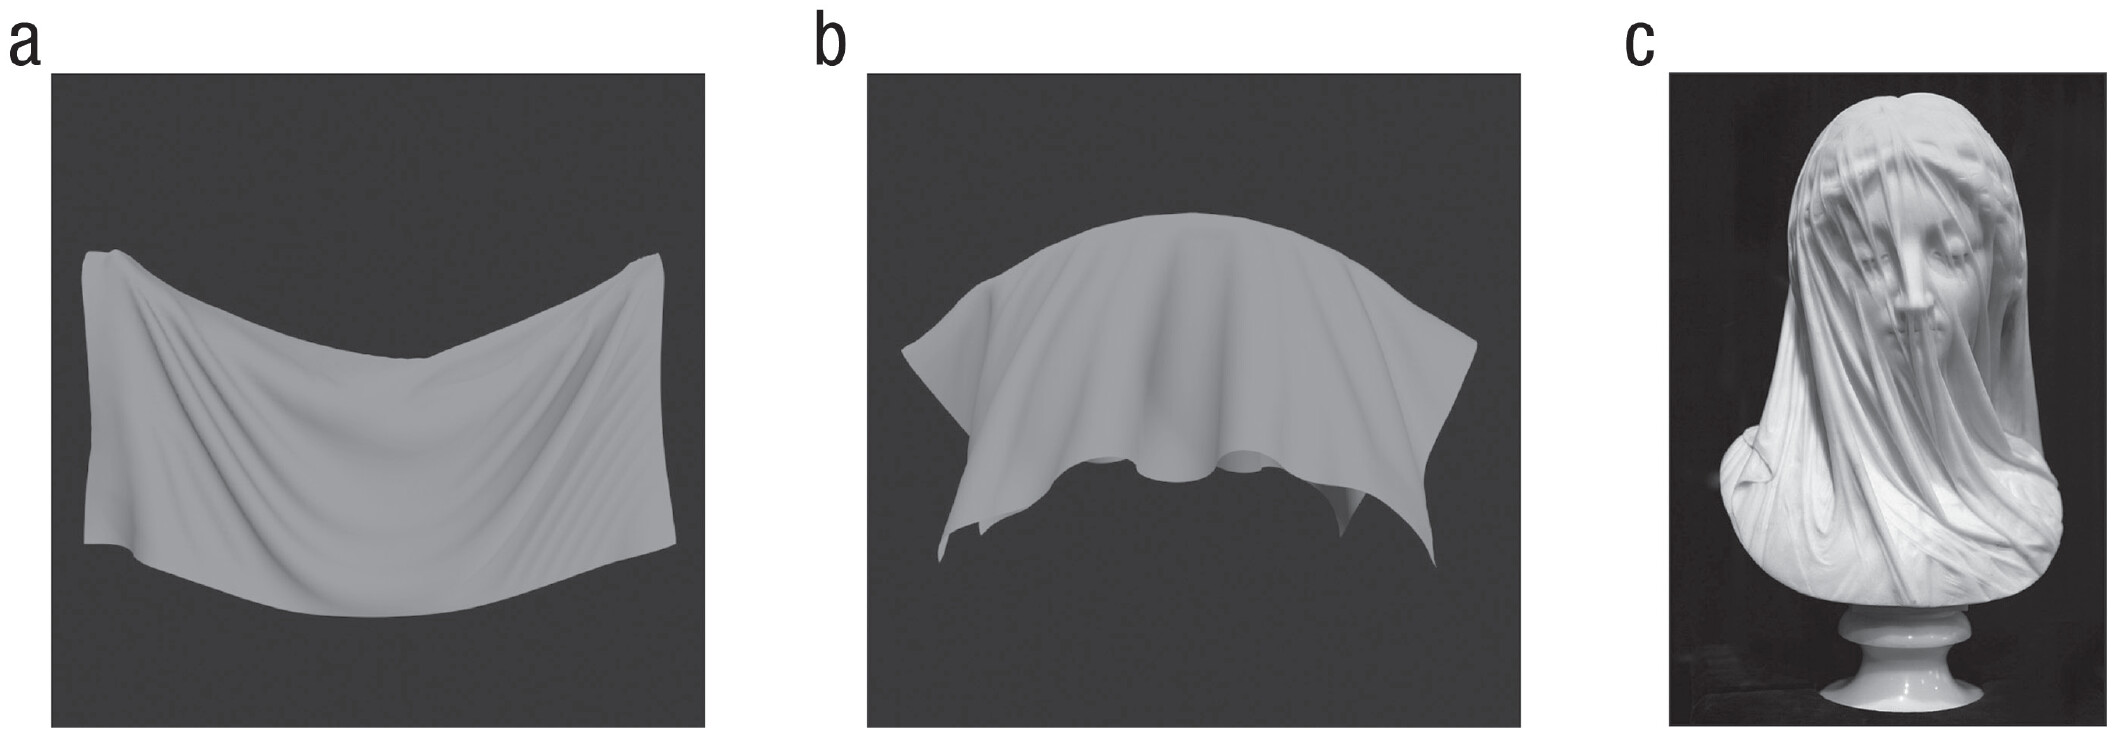
\includegraphics[width=\textwidth]{figures/PsychSci2023/fig1_cloth_statues.jpeg}
    \caption
    {(a) A cloth-covered object where the top curved section may reflect only the folds of the cloth, caused by gravity. (b) An example in which the top curved section must reflect the structure of the underlying object. (c) The “Veiled Virgin,” an example of a sculpture where observers can readily indicate which contours reflect the object versus soft material \protect{\parencite{phillips_veiled_2020}}.}
    \label{fig:PsychSci2023_1}
\end{figure}

%%%%%%%%%%%%%%%%%%%%%%%%%%%%%%%%%%%%%%%%%%%%%%%%%%%%%%%%%%%%%%%%%%%%%%%%%%%
\section{The Current Study}
%%%%%%%%%%%%%%%%%%%%%%%%%%%%%%%%%%%%%%%%%%%%%%%%%%%%%%%%%%%%%%%%%%%%%%%%%%%

The current project established that cloth physics is taken into account during visual perception itself, using multiple experimental paradigms, each of which had two features that to our knowledge have not been explored in past studies (e.g., \cite{phillips_veiled_2020, ullman_draping_2019, yildirim_perceiving_2016}). First, whereas past studies asked for overt judgments about which image contours were which, we employed objective performance-based measures. Second, whereas drawing the cloth/object distinction was the entire explicit goal in past tasks, here this distinction was always entirely task irrelevant. Expts.~1a to 1d explored cloth physics in visual working memory, using change detection, and Expts.~2a and 2b explored cloth physics in visual attention, using probe comparison (inspired by object-based attention studies).

This study was performed in line with the principles of the Declaration of Helsinki. All experimental methods and procedures were approved by the Yale University Institutional Review Board. Informed consent was obtained from all individual participants included in the study.

%%%%%%%%%%%%%%%%%%%%%%%%%%%%%%%%%%%%%%%%%%%%%%%%%%%%%%%%%%%%%%%%%%%%%%%%%%%
\section{Experiment 1a: Sequential Change Detection}
%%%%%%%%%%%%%%%%%%%%%%%%%%%%%%%%%%%%%%%%%%%%%%%%%%%%%%%%%%%%%%%%%%%%%%%%%%%

Observers saw two images of cloth-covered objects appear quickly, one after the other, and simply had to detect whether the two raw images were identical. As depicted in \cref{fig:PsychSci2023_2}a, image changes could involve either (a) a new draping of the cloth (as if the cloth were thrown over the same object again, with substantive changes to cloth regions) or (b) changing the object under the cloth (with substantive changes to object regions). Critically, the sheer amount of visual change was always greater in the first condition than the second --- in terms of both the brute number of pixels changed and also the degree of higher-level feature change (as quantified from relatively late layers in a convolutional neural network trained for object recognition; VGG16; \cite{simonyan_very_2015}). We expected better detection for changes to object regions versus cloth regions, despite the greater degree of visual change in the latter.

\begin{figure}
    \centering
    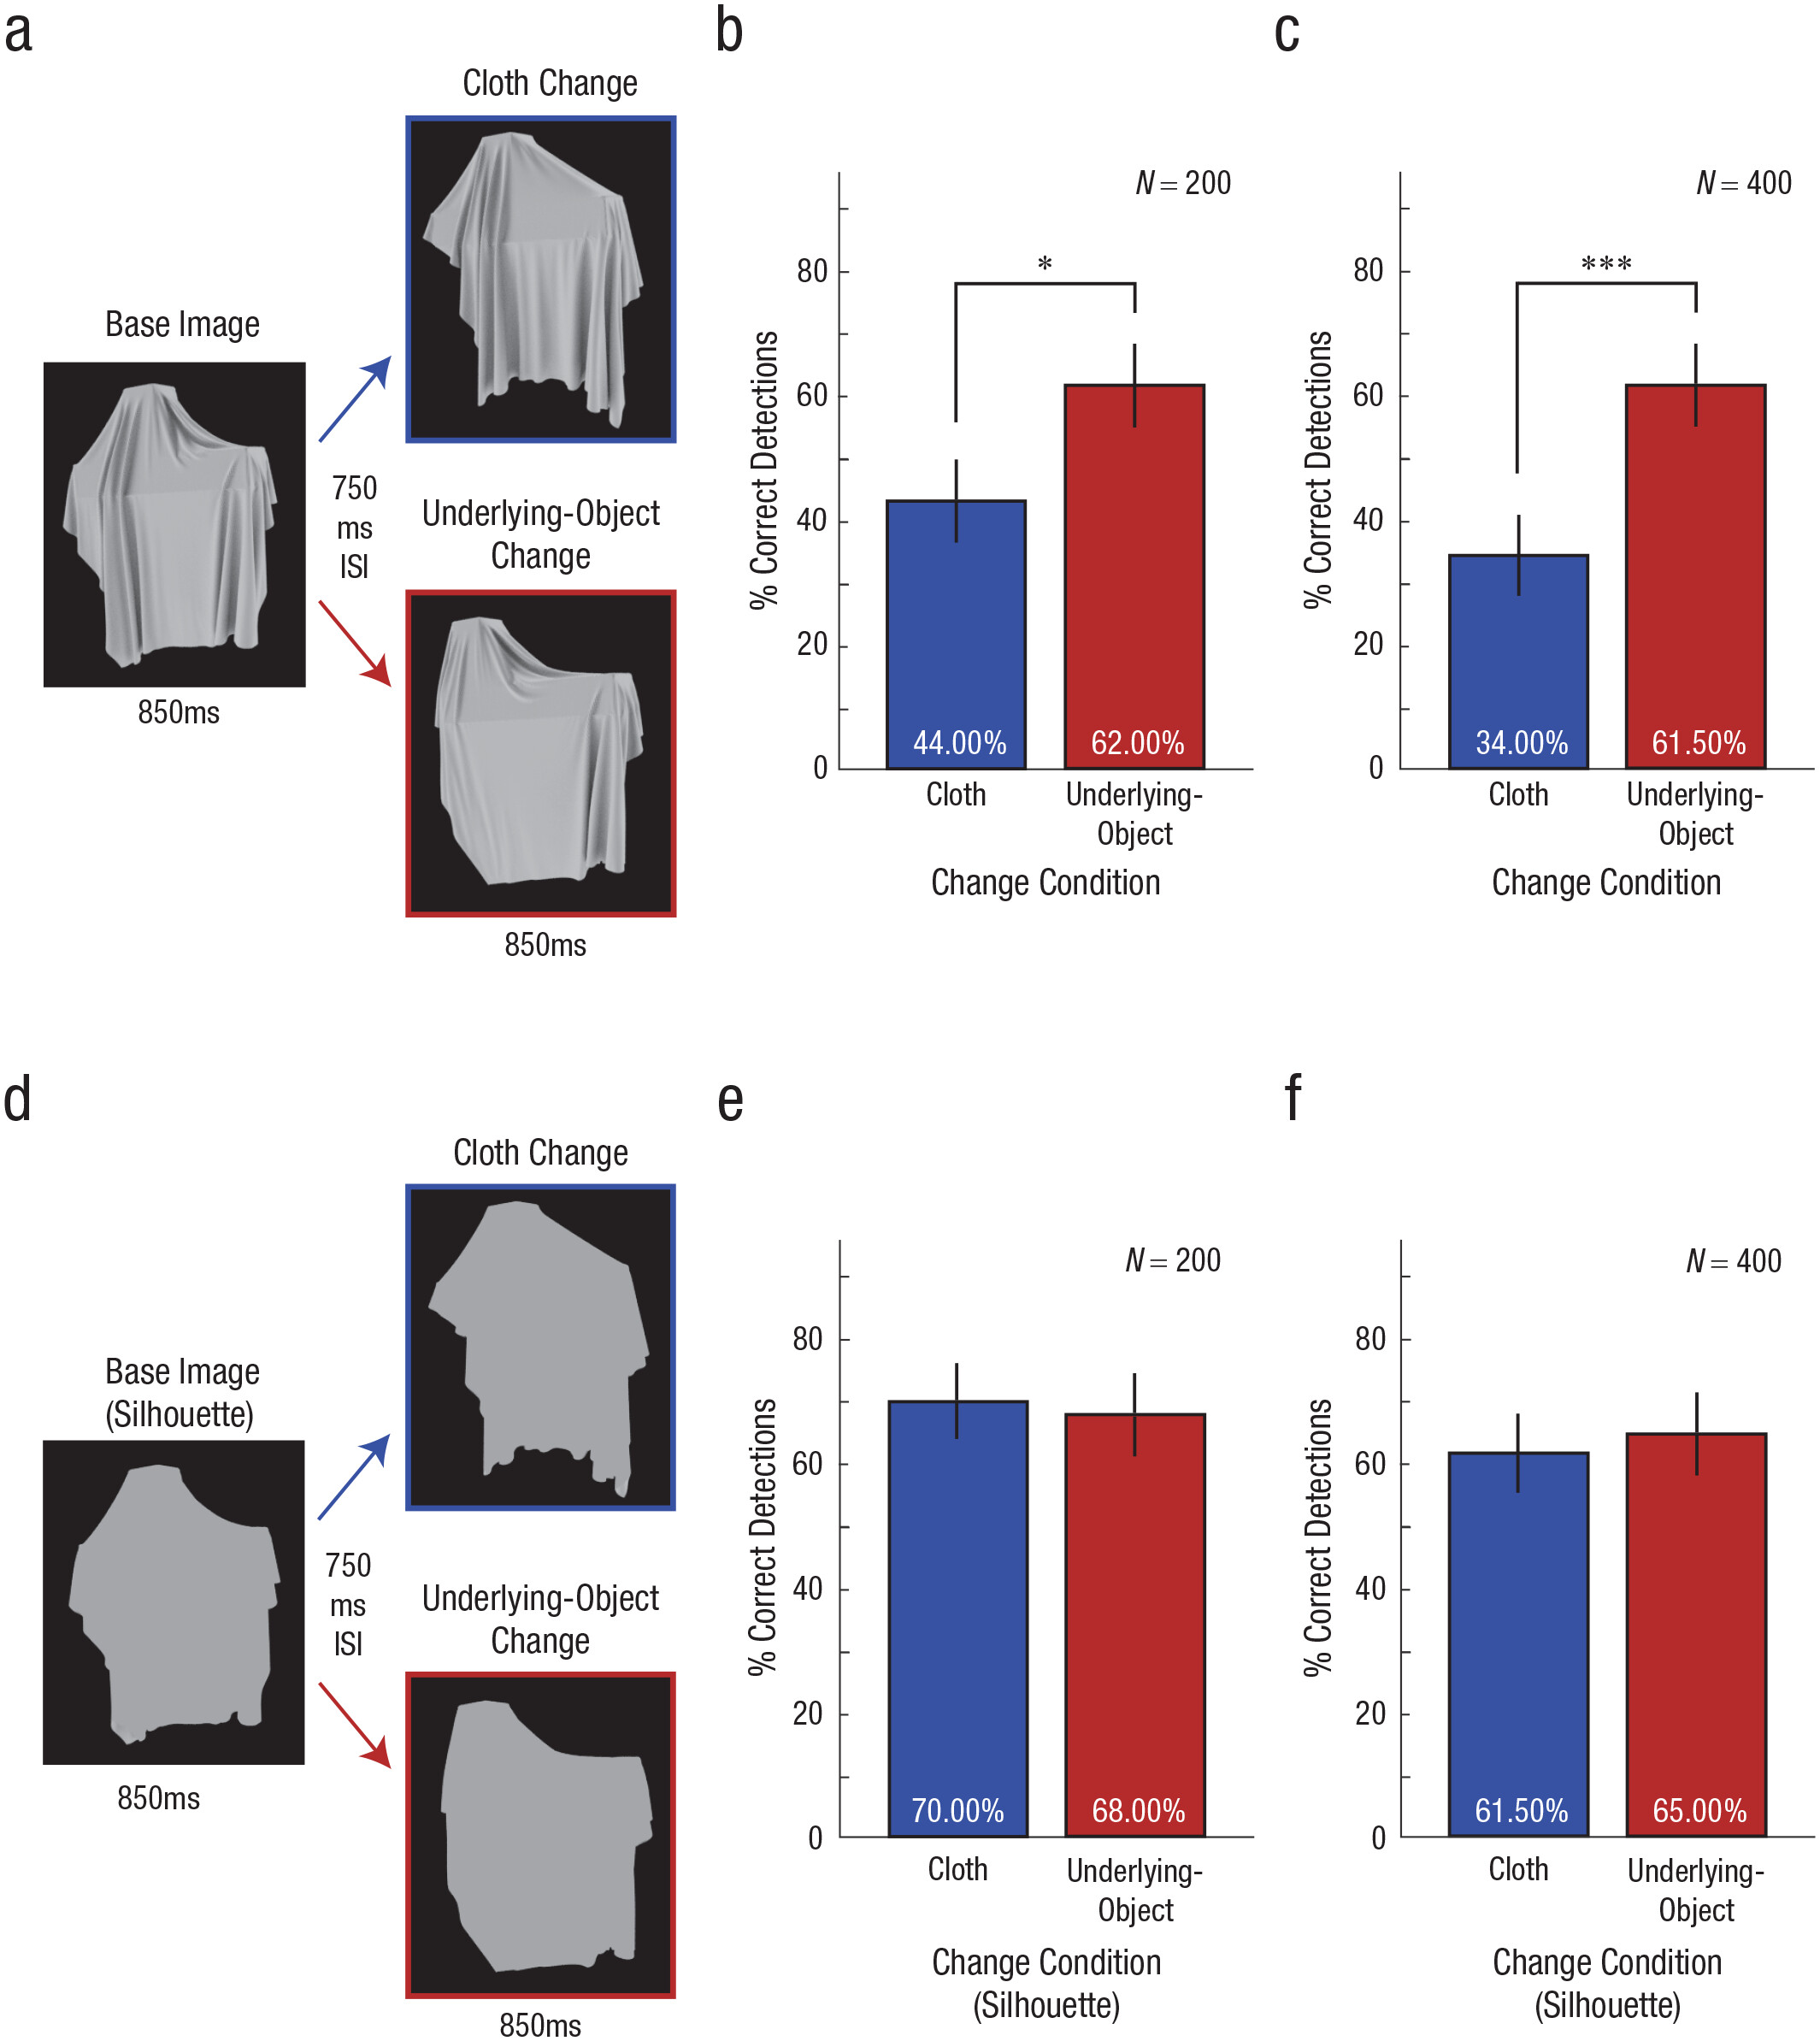
\includegraphics[width=\textwidth]{figures/PsychSci2023/fig2_experiment1.jpeg}
    \caption
    {(a) Depictions of the two key conditions in Expts.~1a and 1b: Images could undergo changes either to the underlying objects or to the superficial folds of the cloths. (b) Average accuracy in each condition of Expt.~1a. (c) Average accuracy in each condition of Expt.~1b. (d) Depictions of the matched key conditions from Expts.~1c and 1d. (e) Average accuracy in each condition of Expt.~1c. (f) Average accuracy in each condition of Expt.~1d. In all graphs, error bars depict \qty{90}{\percent} confidence intervals. Asterisks indicate significant differences between conditions ($^{*}p < .05$, $^{***}p < .001$). ISI = interstimulus interval.}
    \label{fig:PsychSci2023_2}
\end{figure}

%%%%%%%%%%%%%%%%%%%%%%%%%%%%%%%%%%%%%%%%%%%%%%%%%%%%%%%%%%%%%%%%%%%%%%%%%%%
\subsection{Method}
%%%%%%%%%%%%%%%%%%%%%%%%%%%%%%%%%%%%%%%%%%%%%%%%%%%%%%%%%%%%%%%%%%%%%%%%%%%

%%%%%%%%%%%%%%%%%%%%%%%%%%%%%%%%%%%%%%%%%%%%%%%%%%%%%%%%%%%%%%%%%%%%%%%%%%%
\subsubsection{Participants}
%%%%%%%%%%%%%%%%%%%%%%%%%%%%%%%%%%%%%%%%%%%%%%%%%%%%%%%%%%%%%%%%%%%%%%%%%%%

Two hundred observers (79 female; mean age = 24.55~years) participated for monetary compensation using the Prolific online platform \parencite{palan_prolificacsubject_2018}, and this preregistered sample size was determined before data collection began. Observers were excluded (with replacement) according to preregistered criteria if they reported (in response to postexperimental debriefing questions) that the total number of images they saw appear on screen throughout the entire session was anything other than two images ($n = 8$) or if they took longer than \qty{10}{\second} to respond ($n = 22$). All reported experiments employed protocols that were reviewed and approved by the Yale University Institutional Review Board.

%%%%%%%%%%%%%%%%%%%%%%%%%%%%%%%%%%%%%%%%%%%%%%%%%%%%%%%%%%%%%%%%%%%%%%%%%%%
\subsubsection{Apparatus}
%%%%%%%%%%%%%%%%%%%%%%%%%%%%%%%%%%%%%%%%%%%%%%%%%%%%%%%%%%%%%%%%%%%%%%%%%%%

After agreeing to participate, observers were redirected to a website where stimulus presentation and data collection were controlled via custom software written using a combination of HTML, Cascading Style Sheets (CSS), JavaScript, Hypertext Preprocessor, and the JsPsych libraries \parencite{de_leeuw_jspsych_2015}. Observers completed the experiment on either a laptop or desktop computer. (Because the experiment was rendered on observers’ own web browsers, viewing distance, screen size, and display resolutions could vary dramatically, so we report stimulus dimensions below using pixel values.)

%%%%%%%%%%%%%%%%%%%%%%%%%%%%%%%%%%%%%%%%%%%%%%%%%%%%%%%%%%%%%%%%%%%%%%%%%%%
\subsubsection{Stimuli}
%%%%%%%%%%%%%%%%%%%%%%%%%%%%%%%%%%%%%%%%%%%%%%%%%%%%%%%%%%%%%%%%%%%%%%%%%%%

All text, across the instructions and prompts, was presented in a modified version of jsPsych’s default CSS style: light gray (No. D3D3D3~\legendbox{D3D3D3}) text (on a black background) drawn in the Open Sans font, presented at a font size of 18 pixels.
A single Tetris-like object was first created in Blender (Version 2.83; \prettyurl{https://www.blender.org/}), with a $1.2 \times 0.2 \times \qty{0.2}{\meter}$ rectangular prism for a trunk and a $0.4 \times 0.2 \times \qty{0.2}{\meter}$ rectangular prism for a branch. These two prisms were then used to construct six base-objects by first positioning the branch at a \qty{0.05}{\meter} offset from the center of the trunk and then randomly rotating the resulting object (six separate times) along its $x$, $y$, and $z$ axes. Six corresponding modified-objects were then created by holding these rotations constant but shifting the branches to have a \qty{0.35}{\meter} offset (rather than only a \qty{0.05}{\meter} offset) from the center of the trunk.

Objects were depicted with white cloths draped over them (on a black background); this draping was simulated by a particle-based physics engine (Nvidia FleX; \cite{macklin_unified_2014}). The base-object was centered at the origin, with a piece of cloth mesh dropped from a height ($h$) of \qty{1.0}{\meter} from one of 10 possible angles (0.2, 0.4, 0.6, 0.8, 1.0, 1.2, 1.4, 1.6, 1.8, and \qty{2.0}{\radian}). The cloth was simulated as a grid of particles connected to each other by massless springs that collectively simulated stiffness; the cloth itself was $64\times64$ particles (each particle having a radius of \qty{0.01}{\meter}), and cloth mass and all stiffness values (bending, shearing, stretching) were held at a constant of 1.0. The initial velocity and position of the cloth mesh differed according to each angle ($\alpha$): The initial velocity of the cloth ($v_x, v_y, v_z$) was set to be $(1.8\cos(\alpha), 1.8\sin(\alpha), 0)$, and the initial position of the cloth ($p_x, p_y, p_z$) was $(c_x - 0.8v_x\sqrt{2h \times 9.8}, c_y - 0.8v_y\sqrt{2h \times 9.8}, 0)$, where $c_x$ and $c_y$ refer to the $x$ and $y$ positions, respectively, of the base-object’s center of mass. During the simulation, the cloth mesh unfolded over 200 consecutive time steps under the influence of gravity, and each time step (frame) was 1/\qty{60}{\second}. The output of the simulation from the last time step (i.e., 200th frame) was rendered in grayscale via Blender (on a black $400\times 400$-pixel background), and the visible cloth shapes (as in the examples from \cref{fig:PsychSci2023_2}a) were presented with an average area of $132.89\times 241$ pixels, with widths ranging from 104 to 172 pixels and heights ranging from 209 to 267 pixels --- these values varied on the basis of the specific orientation of each base-object.

Six corresponding redraped-objects were then created from the base-objects by holding the rotations and branch positions constant but redraping the cloth from a different angle --- which in practice produced different superficial cloth shapes (as in the contrast between the base image and the cloth-change panels of \cref{fig:PsychSci2023_2}a).

%%%%%%%%%%%%%%%%%%%%%%%%%%%%%%%%%%%%%%%%%%%%%%%%%%%%%%%%%%%%%%%%%%%%%%%%%%%
\subsubsection{Procedure and design}
%%%%%%%%%%%%%%%%%%%%%%%%%%%%%%%%%%%%%%%%%%%%%%%%%%%%%%%%%%%%%%%%%%%%%%%%%%%

Observers each viewed a single trial during which two images were presented, one after the other, for \qty{850}{\milli\second} each (separated by a \qty{750}{\milli\second} blank interval). Images appeared 170 pixels away from the center of the screen (as measured from the center of the image), and each image could appear in one of four locations (and never with both images appearing in the same location) --- either to the upper right (\qty{45}{\degree}), the lower right (\qty{135}{\degree}), the lower left (\qty{225}{\degree}), or the upper left (\qty{315}{\degree}) of the screen’s center. Their task (as instructed before the images were presented) was simply to indicate via a key press whether the two images were identical. Both images consisted of cloth-covered objects as described above. On cloth-change trials, the second image was of a redraped-object. On underlying-object-change trials, the second image was of a cloth-covered modified-object. Examples of both trial types are depicted in \cref{fig:PsychSci2023_2}a.

Critically, the magnitude of visual change on a cloth-change trial was always \textit{greater} than on its corresponding underlying-object-change trial (where these two trials were viewed by different observers). This was always true in terms of both (a) the number of changed pixels in the images themselves and (b) the change in higher-level visual features, quantified by calculating squared Euclidean distance in vectorized feature-activation maps from the second-to-last layer (layer fc1) in a convolutional neural network pretrained for image classification and detection (VGG16; \cite{simonyan_very_2015}) --- with average distances of \num{7459.15} for cloth-change trials and \num{5630.75} for underlying-object-change trials. (And Fourier analyses also revealed no systematic spatial frequency differences across the images in cloth-change trials vs. their corresponding images in underlying-object-change trials.)

%%%%%%%%%%%%%%%%%%%%%%%%%%%%%%%%%%%%%%%%%%%%%%%%%%%%%%%%%%%%%%%%%%%%%%%%%%%
\subsection{Results}
%%%%%%%%%%%%%%%%%%%%%%%%%%%%%%%%%%%%%%%%%%%%%%%%%%%%%%%%%%%%%%%%%%%%%%%%%%%

As depicted in \cref{fig:PsychSci2023_2}b, changes were detected much more accurately on underlying-object-change trials (\qty{62.00}{\percent}) compared with cloth-change trials (\qty{44.00}{\percent}), $\chi^2\,(N = 200) = 6.50,\,p = .011$, effect-size index $w = .18$.

%%%%%%%%%%%%%%%%%%%%%%%%%%%%%%%%%%%%%%%%%%%%%%%%%%%%%%%%%%%%%%%%%%%%%%%%%%%
\section[Experiment 1b: Sequential Change Detection (Direct Replication)]{Experiment 1b: Sequential Change Detection \\ (Direct Replication)}
%%%%%%%%%%%%%%%%%%%%%%%%%%%%%%%%%%%%%%%%%%%%%%%%%%%%%%%%%%%%%%%%%%%%%%%%%%%
%%%%%%%%%%%%%%%%%%%%%%%%%%%%%%%%%%%%%%%%%%%%%%%%%%%%%%%%%%%%%%%%%%%%%%%%%%%
\subsection{Method}
%%%%%%%%%%%%%%%%%%%%%%%%%%%%%%%%%%%%%%%%%%%%%%%%%%%%%%%%%%%%%%%%%%%%%%%%%%%

Given the importance of direct replications, we reran the same experiment on a larger group of 400 independent observers from the same pool (145 female; mean age = 25.89~years). This preregistered sample size was chosen to be exactly twice that from Expt.~1a and, again, excluded observers (with replacement) according to the same two preregistered criteria ($n = 19$ and $n = 28$, respectively).

%%%%%%%%%%%%%%%%%%%%%%%%%%%%%%%%%%%%%%%%%%%%%%%%%%%%%%%%%%%%%%%%%%%%%%%%%%%
\subsection{Results}
%%%%%%%%%%%%%%%%%%%%%%%%%%%%%%%%%%%%%%%%%%%%%%%%%%%%%%%%%%%%%%%%%%%%%%%%%%%

As depicted in \cref{fig:PsychSci2023_2}c, the results conformed to the same pattern as in Expt.~1a: Changes were again detected much more accurately on underlying-object-change trials (\qty{61.50}{\percent}) compared with cloth-change trials (\qty{34.00}{\percent}), $\chi^2\,(N = 400) = 30.31,\,p < .001$, effect-size index $w = 0.28$.

%%%%%%%%%%%%%%%%%%%%%%%%%%%%%%%%%%%%%%%%%%%%%%%%%%%%%%%%%%%%%%%%%%%%%%%%%%%
\section{Experiment 1c: Sequential Change Detection (Silhouettes)}
%%%%%%%%%%%%%%%%%%%%%%%%%%%%%%%%%%%%%%%%%%%%%%%%%%%%%%%%%%%%%%%%%%%%%%%%%%%

The pattern of results observed in Expts.~1a and 1b cannot be explained by brute change magnitude because, by design, there was always greater visual change on cloth-change trials than underlying-object-change trials. But it could be predicted by attention and/or memory prioritizing “deep” object information beyond “superficial” cloth contours. This view also predicts that the observed change-detection patterns should disappear if the cloth/object distinction itself were eliminated in the image. We tested this by presenting stimulus silhouettes, as in \cref{fig:PsychSci2023_2}d.

%%%%%%%%%%%%%%%%%%%%%%%%%%%%%%%%%%%%%%%%%%%%%%%%%%%%%%%%%%%%%%%%%%%%%%%%%%%
\subsection{Method}
%%%%%%%%%%%%%%%%%%%%%%%%%%%%%%%%%%%%%%%%%%%%%%%%%%%%%%%%%%%%%%%%%%%%%%%%%%%

This experiment was identical to Expt.~1a, except as noted. A new set of 200 observers from the same pool (71 female; mean age = 23.67~years) was recruited, once again excluding observers (with replacement) according to the same two preregistered criteria ($n = 6$ and $n = 24$, respectively). Stimuli were identical to those used in Expt.~1a, except that they were presented as silhouettes (with the internal areas filled with a single shade of gray equal to that of the cloth resting directly on the object surface; No. A4A4A4~\legendbox{A4A4A4}).


%%%%%%%%%%%%%%%%%%%%%%%%%%%%%%%%%%%%%%%%%%%%%%%%%%%%%%%%%%%%%%%%%%%%%%%%%%%
\subsection{Results}
%%%%%%%%%%%%%%%%%%%%%%%%%%%%%%%%%%%%%%%%%%%%%%%%%%%%%%%%%%%%%%%%%%%%%%%%%%%

As depicted in \cref{fig:PsychSci2023_2}e, change detection did not differ on underlying-object-change trials (\qty{68.00}{\percent}) compared with cloth-change trials (\qty{70.00}{\percent}). $\chi^2\,(N = 200) = .09,\,p < .760$, effect-size index $w = .02$ --- and this null effect (the slight numerical difference for which was actually in the opposite direction) differed from the robust effect observed in Expt.~1a (odds ratio = 2.28, $p < .05$).

%%%%%%%%%%%%%%%%%%%%%%%%%%%%%%%%%%%%%%%%%%%%%%%%%%%%%%%%%%%%%%%%%%%%%%%%%%%
\section[Experiment 1d: Seq. Change Detection (Silhouettes, Dir. Replication)]{Experiment 1d: Sequential Change Detection (Silhouettes, Direct Replication)}
%%%%%%%%%%%%%%%%%%%%%%%%%%%%%%%%%%%%%%%%%%%%%%%%%%%%%%%%%%%%%%%%%%%%%%%%%%%

%%%%%%%%%%%%%%%%%%%%%%%%%%%%%%%%%%%%%%%%%%%%%%%%%%%%%%%%%%%%%%%%%%%%%%%%%%%
\subsection{Method}
%%%%%%%%%%%%%%%%%%%%%%%%%%%%%%%%%%%%%%%%%%%%%%%%%%%%%%%%%%%%%%%%%%%%%%%%%%%
Given the importance of direct replications, we reran Expt.~1c on a larger group of 400 independent observers from the same pool (160 female; mean age = 26.20~years). This preregistered sample size was chosen to be exactly twice that from Expt.~1c (and equal to that from Expt.~1b), again excluding observers (with replacement) according to the same two preregistered criteria ($n = 21$ and $n = 38$, respectively).

%%%%%%%%%%%%%%%%%%%%%%%%%%%%%%%%%%%%%%%%%%%%%%%%%%%%%%%%%%%%%%%%%%%%%%%%%%%
\subsection{Results}
%%%%%%%%%%%%%%%%%%%%%%%%%%%%%%%%%%%%%%%%%%%%%%%%%%%%%%%%%%%%%%%%%%%%%%%%%%%

As depicted in \cref{fig:PsychSci2023_2}f, change detection did not differ on underlying-object-change trials (\qty{65.00}{\percent}) compared with cloth-change trials (\qty{61.50}{\percent}), $\chi^2\,(N = 400) = .53,\,p = .468$, effect-size index $w = .04$ --- and this null effect differed from the robust difference observed in Expt.~1b (odds ratio = 2.67, $p < .001$).


%%%%%%%%%%%%%%%%%%%%%%%%%%%%%%%%%%%%%%%%%%%%%%%%%%%%%%%%%%%%%%%%%%%%%%%%%%%
\section{Experiment 2a: Simultaneous Probe Comparison}
%%%%%%%%%%%%%%%%%%%%%%%%%%%%%%%%%%%%%%%%%%%%%%%%%%%%%%%%%%%%%%%%%%%%%%%%%%%

Performance in the previous experiments seemed to depend not on the image properties themselves but rather on how various contours were represented as a function of intuitive physics --- in terms of reflecting deep object contours versus superficial cloth contours. But are these representations formed during online perception or only later --- perhaps during retrieval from memory, after the images themselves have disappeared? We addressed this using a paradigm in which the relevant information is always simultaneously visible on the display. Inspired by studies of “same-object (dis)advantages” in object-based attention (e.g., \cite{egly_shifting_1994, marino_role_2005}), we tested this using probe comparison. Two probes appeared atop an image of a cloth-covered object (as depicted in \cref{fig:PsychSci2023_3}a), and observers simply reported whether they were identical. Both probes always appeared on the images, but we predicted that performance would vary on the basis of whether they both appeared on object regions (vs. one appearing on a cloth region).

\begin{figure}
    \centering
    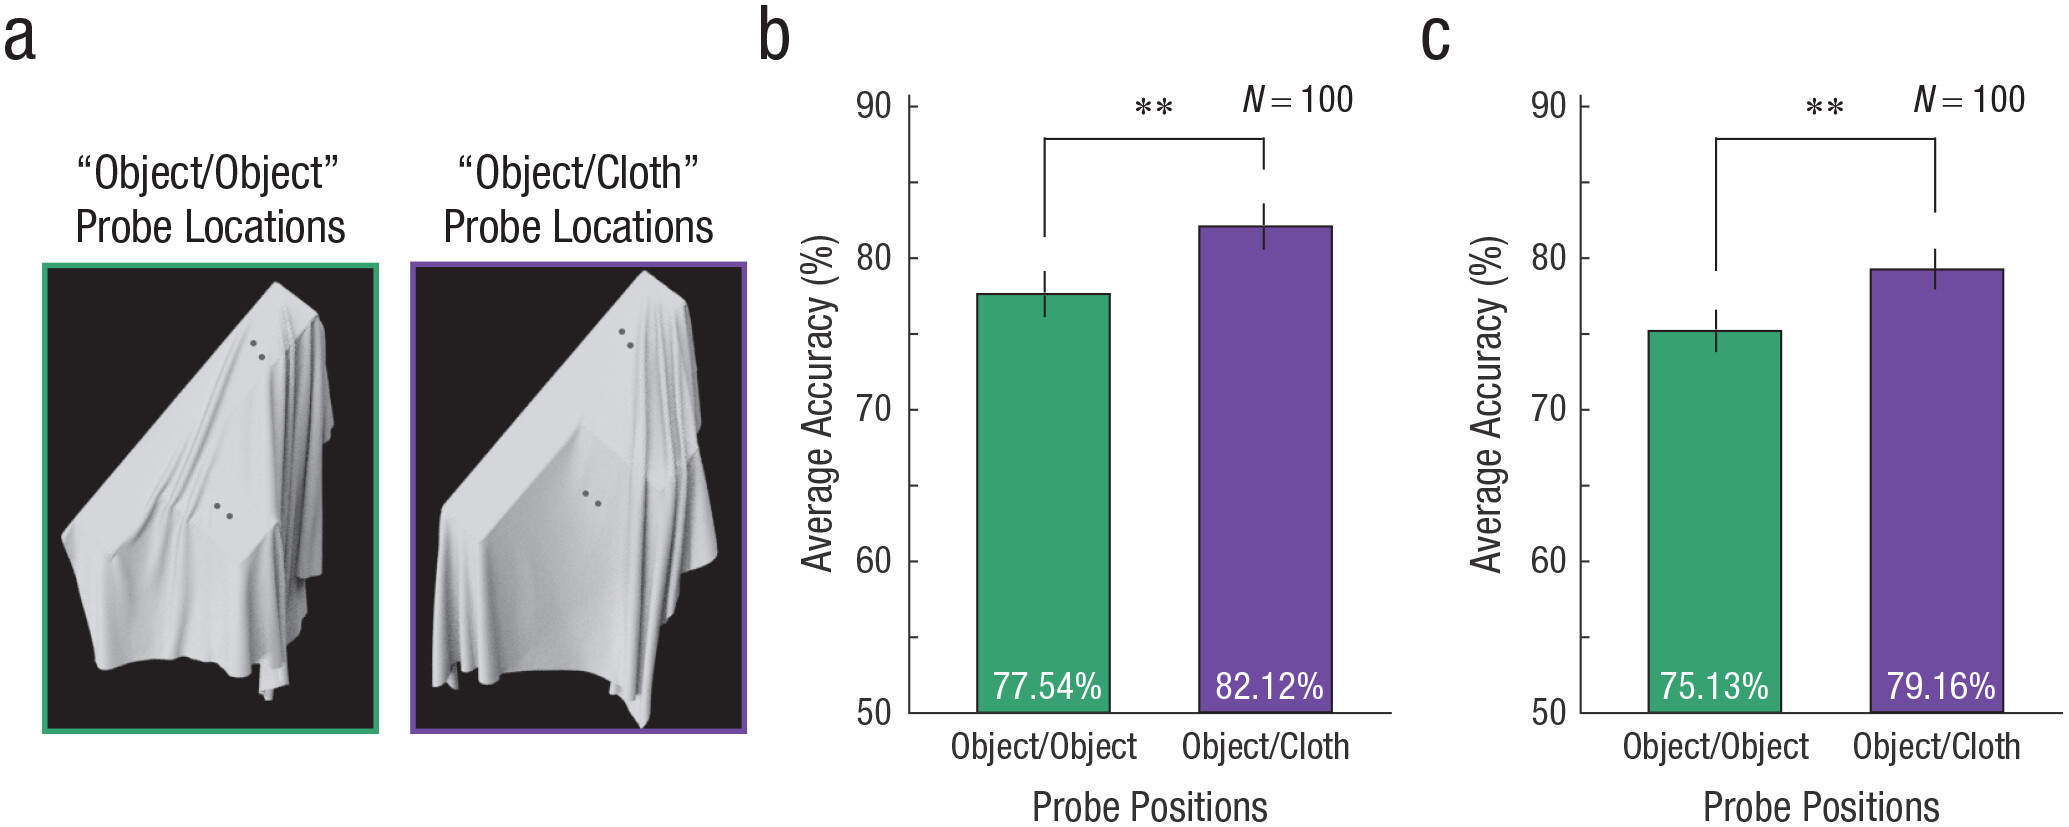
\includegraphics[width=\textwidth]{figures/PsychSci2023/fig3_experiment2.jpeg}
    \caption
    { (a) Depictions of the two key conditions in Expts.~2a and 2b: The two probes could both appear on object regions, or one could appear on a cloth region. (b) Average accuracy for each probe position in Expt.~2a. (c) Average accuracy for each probe position in Expt.~2b. In both graphs, error bars depict \qty{95}{\percent} confidence intervals after subtracting shared variance. Asterisks indicate significant differences between conditions ($^{**}p < .01$).}
    \label{fig:PsychSci2023_3}
\end{figure}

%%%%%%%%%%%%%%%%%%%%%%%%%%%%%%%%%%%%%%%%%%%%%%%%%%%%%%%%%%%%%%%%%%%%%%%%%%%
\subsection{Method}
%%%%%%%%%%%%%%%%%%%%%%%%%%%%%%%%%%%%%%%%%%%%%%%%%%%%%%%%%%%%%%%%%%%%%%%%%%%

%%%%%%%%%%%%%%%%%%%%%%%%%%%%%%%%%%%%%%%%%%%%%%%%%%%%%%%%%%%%%%%%%%%%%%%%%%%
\subsubsection{Participants}
%%%%%%%%%%%%%%%%%%%%%%%%%%%%%%%%%%%%%%%%%%%%%%%%%%%%%%%%%%%%%%%%%%%%%%%%%%%

One hundred observers (33 female; mean age = 24.94~years) participated for monetary compensation using the Prolific online platform \parencite{palan_prolificacsubject_2018}. This preregistered sample size was determined before data collection began.

%%%%%%%%%%%%%%%%%%%%%%%%%%%%%%%%%%%%%%%%%%%%%%%%%%%%%%%%%%%%%%%%%%%%%%%%%%%
\subsubsection{Stimuli}
%%%%%%%%%%%%%%%%%%%%%%%%%%%%%%%%%%%%%%%%%%%%%%%%%%%%%%%%%%%%%%%%%%%%%%%%%%%

Eight underlying objects (four base-objects and four corresponding modified-objects) were generated and then covered with cloths as in the previous experiments, except without any constraints involving change magnitudes. Each probe consisted of two 3-pixel gray dots (No. 5E5E5E~\legendbox{5E5E5E}) that were initially vertically aligned, with their centers 5 pixels apart. During their actual presentation, each probe could then be rotated by \qty{30}{\degree}, \qty{50}{\degree}, \qty{310}{\degree}, or \qty{330}{\degree}. Two such probes were then placed on each cloth-covered object stimulus during each trial, as described below.

%%%%%%%%%%%%%%%%%%%%%%%%%%%%%%%%%%%%%%%%%%%%%%%%%%%%%%%%%%%%%%%%%%%%%%%%%%%
\subsubsection{Procedure and design}
%%%%%%%%%%%%%%%%%%%%%%%%%%%%%%%%%%%%%%%%%%%%%%%%%%%%%%%%%%%%%%%%%%%%%%%%%%%

Using the same apparatus from the previous experiments, we began each trial with the image (of an object covered by a cloth) appearing in a random location. After \qty{350}{\milli\second}, two probes appeared on the image, and \qty{300}{\milli\second} later, both the probes and the images disappeared. Observers then reported whether the two probes were identical (i.e., whether the dot pair in each probe had the same degree of rotation) --- where nonidentical probe orientations always differed by \qty{20}{\degree}. On object/object trials, both probes were located on object regions (in one of four fixed image-relative locations). On corresponding object/cloth trials, one probe was located on an object region, whereas the other was located on a cloth region --- always equating the interprobe distances and directions across these two trial types, as depicted in \cref{fig:PsychSci2023_3}a (and these equated locations also prevented any differential influence of horizontal vs. vertical arrangements; cf. \cite{chen_when_2019}).

Each observer completed 32 trials, presented in a different random order for each observer: 4 base-objects $\times$ 2 conditions (object/object vs. object/cloth) $\times$ 2 possible base probe rotations (\qty{30}{\degree}/\qty{50}{\degree} or \qty{310}{\degree}/\qty{330}{\degree}) × 2 probe rotation matching possibilities (identical vs. different). Observers were excluded (with replacement) according to two preregistered criteria. First, in a postexperimental debriefing phase, observers self-reported how well they paid attention (on a continuous scale ranging from 1 = \textit{very distracted} to 100 = \textit{very focused}), and we excluded observers who self-reported an attention level below 70 ($n = 12$). Second, we also excluded observers whose mean accuracy was lower than \qty{60}{\percent} (who were not already excluded via Criterion 1; $n = 35$). Individual trials with response times 2 or more standard deviations away from the mean response time of all observers were also excluded (on average, 0.97 trials/observer).

%%%%%%%%%%%%%%%%%%%%%%%%%%%%%%%%%%%%%%%%%%%%%%%%%%%%%%%%%%%%%%%%%%%%%%%%%%%
\subsection{Results}
%%%%%%%%%%%%%%%%%%%%%%%%%%%%%%%%%%%%%%%%%%%%%%%%%%%%%%%%%%%%%%%%%%%%%%%%%%%

Our preregistered analysis plan made no prediction as to the specific direction of a performance difference across conditions, because past studies have observed both same-object advantages and same-object disadvantages depending on subtle stimulus differences (for a review, see \cite{chen_solving_2015}). (Our underlying theoretical question was only whether the visual system was drawing the cloth/object distinction --- and so a reliable, systematic difference in either direction serves to support that possibility.) As depicted in Figure \cref{fig:PsychSci2023_3}b, probe comparison performance was better on object/cloth trials (\qty{82.12}{\percent}) compared with object/object trials (\qty{77.54}{\percent}), $t(99) = 3.18,\,p = .002,\,d = 0.32$.

%%%%%%%%%%%%%%%%%%%%%%%%%%%%%%%%%%%%%%%%%%%%%%%%%%%%%%%%%%%%%%%%%%%%%%%%%%%
\section{Experiment 2b: Simultaneous Probe Comparison (Direct Replication)}
%%%%%%%%%%%%%%%%%%%%%%%%%%%%%%%%%%%%%%%%%%%%%%%%%%%%%%%%%%%%%%%%%%%%%%%%%%%

%%%%%%%%%%%%%%%%%%%%%%%%%%%%%%%%%%%%%%%%%%%%%%%%%%%%%%%%%%%%%%%%%%%%%%%%%%%
\subsection{Method}
%%%%%%%%%%%%%%%%%%%%%%%%%%%%%%%%%%%%%%%%%%%%%%%%%%%%%%%%%%%%%%%%%%%%%%%%%%%

Given the importance of direct replications, we reran the same experiment with an independent group of 100 observers from the same pool (40 female; mean age = 24.15~years). This preregistered sample size was chosen to match that of Expt.~2a. Using the same preregistered criteria, we excluded observers on the basis of self-reported attention levels ($n = 8$) and mean accuracy ($n = 24$), and we excluded trials on the basis of response time variance (on average, 0.73 trials/observer).

%%%%%%%%%%%%%%%%%%%%%%%%%%%%%%%%%%%%%%%%%%%%%%%%%%%%%%%%%%%%%%%%%%%%%%%%%%%
\subsection{Results}
%%%%%%%%%%%%%%%%%%%%%%%%%%%%%%%%%%%%%%%%%%%%%%%%%%%%%%%%%%%%%%%%%%%%%%%%%%%

As depicted in \cref{fig:PsychSci2023_3}c, probe comparison performance was again better on object/cloth trials (\qty{79.16}{\percent}) compared with object/object trials (\qty{75.13}{\percent}), $t(99) = 2.67,\,p = .009,\,d = .27$.

%%%%%%%%%%%%%%%%%%%%%%%%%%%%%%%%%%%%%%%%%%%%%%%%%%%%%%%%%%%%%%%%%%%%%%%%%%%
\section{General Discussion}
%%%%%%%%%%%%%%%%%%%%%%%%%%%%%%%%%%%%%%%%%%%%%%%%%%%%%%%%%%%%%%%%%%%%%%%%%%%

This study, as in so much of vision science, involves a central contrast between \textit{images} and \textit{percepts}. The raw images used in this study did not explicitly distinguish between those contours reflective of the deep structure of the underlying (covered) objects and those reflective only of the superficial contours of the (covering) cloths themselves. Yet observers’ percepts clearly respected these distinctions, taking into account the intuitive physics of how cloth, gravity, and objects interact, to prioritize some image contours over others.

This study did not aim just to verify that people are able to draw this distinction, because this has been directly demonstrated in other recent work \parencite{phillips_veiled_2020, ullman_draping_2019, yildirim_perceiving_2016}. Rather, we explored what types of mental processes are involved, considering the possibility that the cloth/object distinction is drawn during seeing itself, rather than only higher-level reasoning and decision-making. Thus, our experiments differed from prior intuitive physics studies in two key ways. First, instead of posing explicit questions, we employed subtler performance-based measures, which observers cannot intentionally control. Second, whereas all past studies in this domain directly asked observers about the soft materials and/or the underlying objects, this distinction was always completely task irrelevant here.

These themes were apparent in the results from two converging experimental paradigms (both involving high power and direct replications). In change detection (Expts.~1a–1d), observers were better able to detect image changes that reflected different underlying objects versus changes that reflected only superficial cloth contours --- even though the latter were more visually extreme in multiple ways. These results (which disappeared when using silhouettes) were especially striking, showing not only that attention and memory were drawing the cloth/object distinction (despite its task irrelevance) but also that observers apparently could not stop this --- as they would have performed better had these underlying representations not prioritized the object regions. And in probe comparison (Expts.~2a and 2b), observers’ accuracy when comparing two probes differed depending on probe placement on cloth versus object regions (equating distance and direction) --- despite these categories being task irrelevant. These studies thus demonstrate that a facility with this form of intuitive physics occurs to some degree automatically and incidentally, as a part of seeing such stimuli in the first place. Note that this conclusion is orthogonal to most other recent accounts of intuitive physics, such as those that appeal to simulation, or notions of a “game engine” in the mind (e.g., \cite{battaglia_simulation_2013, hamrick_inferring_2016, ullman_mind_2017}). From that perspective, what the current results demonstrate is that some such simulations are performed in a relatively automatic (or even irresistible) manner during seeing itself, rather than being triggered only by higher-level goals and intentions.

The online testing platform used in these studies involves a population that is diverse along many dimensions (see \cite{palan_prolificacsubject_2018}), but we cannot generalize the current results beyond this population, and further studies will be required to test whether such effects also occur in people who are not frequent participants in online studies. Similarly, although the stimuli used in the studies were rendered in photorealistic ways, they still used relatively simple “‘Tetris-like’” stimuli under the cloths (in order to allow for precise and systematic changes), and so further research will be necessary in order to generalize such results to other classes of cloth-covered stimuli --- as well as to soft materials of varying thicknesses and degrees of stiffness.

Our results can be understood by analogy to the perception of lightness. When raw images are viewed, some image luminance information is highlighted in visual processing because it is informative about the deeper underlying reflectances of objects --- but other image luminance information is effectively discounted because it reflects (merely) highly variable details of ambient lighting (for a review, see \cite{adelson_lightness_2000}). The current experiments demonstrate the same pattern with cloth physics: When raw images of cloth-covered objects are viewed, some image contours are highlighted in visual processing because they are informative of the deeper underlying object structure --- but other image contours are effectively discounted because they reflect (merely) highly variable details of how the cloth was draped. In perception, attention, and memory, visual processing may not only “discount the illuminant” but also “discount the cloth.” And this type of dynamic during visual processing may be just as integral to intuitive physics in our mental lives as is higher-level reasoning about physics.


%%%%%%%%%%%%%%%%%%%%%%%%%%%%%%%%%%%%%%%%%%%%%%%%%%%%%%%%%%%%%%%%%%%%%%%%%%%
\section{Acknowledgements}
%%%%%%%%%%%%%%%%%%%%%%%%%%%%%%%%%%%%%%%%%%%%%%%%%%%%%%%%%%%%%%%%%%%%%%%%%%%

For helpful conversation and/or comments on earlier drafts of this article, we thank the members of both the Yale Perception \& Cognition Lab and the Yale Cognitive \& Neural Computation Lab.